\chapter{Periodicity from photometric measurements} % Main chapter title
\protect\label{chapter:photometry}
\lhead{Chapter 2. \emph{Periodicity of {\prox} from photometric measurements}}

To process the data for all the periodicity studies in this \paperorthesis, {\Firstp} wrote all the associated software
in Python using alternative Lomb-Scargle routines provided by {\scipy} library \citep{jones01}, the {\astroml} library,
\citep{vanderplas12} and the {\gatspy} library, \citep{vanderplas15}, comparing the results. In a few cases the {\scipy}
library version gave division-by-zero errors and similar, hence the other two routines were generally preferred. However
when the {\scipy} library did work, the results tended to agree more with the {\gatspy} routine than the {\astroml}
routine, so in most cases the {\gatspy} routine was used and in all the results and the figures below those from
the {\gatspy} routine were used, unless otherwise noted.
%In some cases, such as with
%the {\asas} and {\hst} measurements described in this section, the results from the three routines were nearly
%identical. However for more ``marginal'' data, the three routines frequently gave significantly different results.

As nearly all previous measurements of periodicity in {\prox} were made using Photometric observations, in this
{\paperorthesis}, before discussing spectroscopic measurements such as with the {\harps} data and the various methods of
analysing the {\ha} lines, {\Firstp} first present results obtained from the Photometric observations for {\prox} taken
from the V-Band (there were no data for the I-Band) of the All Sky Automated Survey (\asas), \citep{pojmanski97}, which
contains data between the periods December 2000 to September 2009.

As indicated by the {\asas} guidelines\footnote{This is described in http://www.astrouw.edu.pl/asas/explanations.html},
with {\prox} set out in the {\asas} data as having magnitude 11 in the V-band, {\Firstp} took the data from the second
aperture (numbered 1 as the apertures are numbered starting at zero). {\FirstP} are only considering the ``best'' (grade
A) data from this aperture, which has 970 points. As some of the observations were overlapping in time, {\Firstp} binned these
to 1 day, which reduced the number of points to 624. {\FirstP} then obtained the periodogram shown in the upper panel of
Fig. \ref{fig:asasexample}. Periods between 20 and 160 days were taken in this case. It is noticeable that there only
two significant peaks, at 82.6 and 106.8 days. There was negligible difference between the results of the three Python
routines used. %(with IDs 142941-6240.7, 142942-6240.8, 142942-6240.7 and 142941-6240.8, these are identical)

{\FirstP} also obtained a periodogram from the {\hst} data discussed in \citealt{benedict92,benedict98} consisting of
171 points obtained between July 1995 and January 1998, later enhanced so the last 18 points extended to January 2001,
obtaining the lower panel of Fig. \ref{fig:asasexample}, again taking between 20 and 160 days. The observation times
were either on separate days, or spaced out evenly throughout a single day with the result that binning this data would
have reduced the data unacceptably, so {\Firstp} did not binning the {\hst} data.

\begin{figure}[!htbp]
\begin{center}
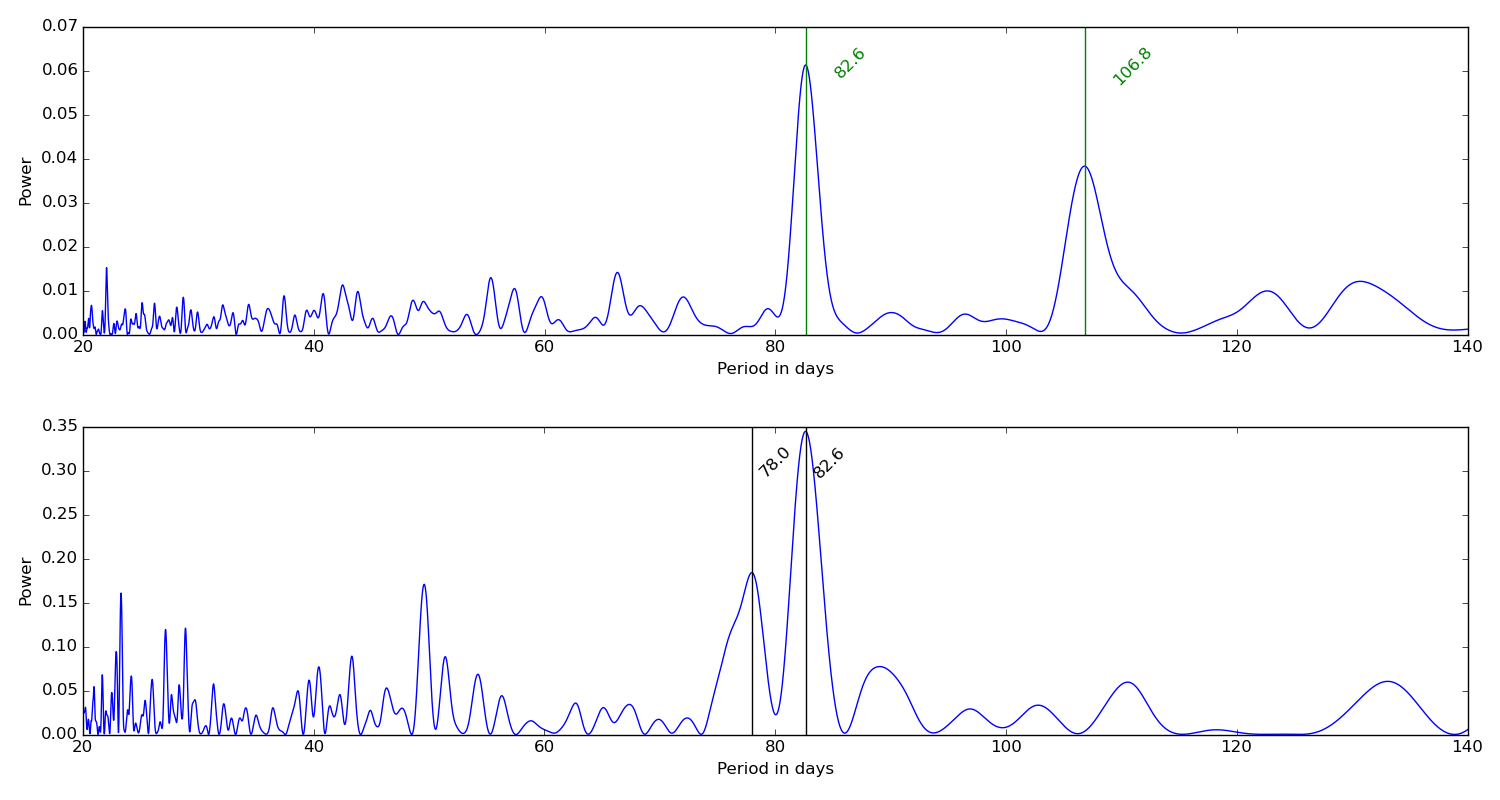
\includegraphics[scale=0.20]{Figures/asashstcomb.png} \\
\end{center}   
\caption{The upper panel is a periodogram from the {\asas} database for {\prox} second aperture, binned to 1 day
  (this reduces the total number from 970 to 624 points), using the {\gatspy} routine examining periods between 20 and
  160 days showing the two strong peaks at 82.6 and 106.8 days. The lower panel is a similar periodogram, also using
  {\gatspy} from the {\hst} data discussed in \citet{benedict98} between July 1995 and January 1998 plus some additional
  points up to January 2001 examining periods showing the a strong peak at 82.6 and a smaller additional peak at 78.0
  days.}
\protect\label{fig:asasexample}
\end{figure}

Although the recommended aperture by {\asas} for {\prox} is the second aperture, {\Firstp} noted the three highest peaks from
each of the apertures and found that all the data gave a first peak of 82.6 $\pm$ 0.1 days, a second peak of 106.5 $\pm$
0.2 days and a much smaller third peak of about 41 days or 68 days.

% and list the results in Table \ref{table:asasperiods}, doing this for the whole of the data and after binning the observations to 0.25 days.
{\FirstP} also examined the other grades of {\asas} data, mostly from ID 142944-6241.0, with a little under half of the
Class A data, 416 points and much higher error rating. All the periodograms from this lower quality data still showed a
strong peak of around 82.5 days, again regardless of which of the three Lomb-Scargle routines were used.

%\begin{table}[!htbp]
%\centering
%\scalebox{0.5}{
%\begin{tabular}{|l|c|c|c|}
%\hline
%Aperture & Peak 1 & Peak 2 & Peak 3 \\\hline
%1 & 83.0 & 106.5 & 40.7 \\
%2 & 82.8 & 106.7 & 40.8 \\
%3 & 82.8 & 106.4 & 68.5 \\
%4 & 82.6 & 106.3 & 68.5 \\
%5 & 82.6 & 106.2 & 68.6 \\\hline
%Mean $\pm$ std & 82.8 $\pm$ 0.2 & 106.4 $\pm$ 0.2 & n/a \\\hline
%1 binned & 82.8 & 106.2 & 130.4 \\
%2 binned & 82.7 & 106.5 & 130.4 \\
%3 binned & 82.7 & 106.3 & 130.3 \\
%4 binned & 82.6 & 106.3 & 130.5 \\
%5 binned & 82.6 & 106.2 & 123.5 \\\hline
%Mean $\pm$ std & 82.7 $\pm$ 0.1 & 106.3 $\pm$ 0.1 & n/a \\\hline
%\end{tabular}}
%\caption{Summary of three strongest periods taken from Class A values in {\asas} dataset for {\prox} from all apertures based upon magnitudes measured
%  between December 2000 and September 2009 with mean and standard deviation for first two. Results are shown for the raw
%data and data binned to 0.25 days in each case.}
%\protect\label{table:asasperiods}
%\end{table}

%\begin{table}[!htbp]
%\centering
%\scalebox{0.75}{
%\begin{tabular}{|l|c|c|c|}
%\hline
%Aperture & Peak 1 & Peak 2 & Peak 3 \\\hline
%1 & 83.2 & 105.7 & 67.9 \\
%2 & 83.0 & 105.3 & 67.6 \\
%3 & 83.3 & 106.0 & 68.4 \\
%4 & 84.0 & 106.1 & 68.5 \\
%5 & 84.2 & 82.4 & 106.0 \\\hline
%Mean $\pm$ std & 83.5 $\pm$ 0.5 && \\\hline
%\end{tabular}}
%\caption{Summary of three strongest periods taken from Class B and lower quality values in {\asas} datasets for {\prox}
%  based upon magnitudes measured between December 2000 and September 2009 with mean and standard deviation for the first.}
%\protect\label{table:asaserrper}
%\end{table}

It is clear that there is consistent agreement between these results with a strong period of 82.6 $\pm$ 0.1 days, in
agreement with the results in \citet{benedict98} and confirmed in \citet{kiraga07}.  The {\asas} data also includes a
reasonably strong additional signal of 106.5 $\pm$ 0.2 days. Taking account of the possibility of this being associated
with some interaction between the main period and some other
period, % as discussed in Section \ref{section:multiperiod},
{\Firstp} considered whether this might be a ``beat'' period between the observation years and the rotational period, as
we noticed the relationship $ \frac{1}{\frac{1}{82.5} - \frac{1}{365.25}} = 106.6 $ and {\Firstp} also noticed that $
\frac{1}{\frac{1}{82.5} + \frac{1}{365.25}} = 67.4 $, which appears as the third peak observed in some of the
periodograms obtained from all the {\asas} apertures.
% It is notable that the {\hst} data does not appear to
% return these periods anywhere, consistent with the fact that the {\hst} is not so limited to the time of year when
% {\prox} may be viewed. REMEMBER THIS SHOULD BE IN DISCUSSION

{\FirstP} also searched for very long periods up to the period spanned by the data in each case, however {\Firstp} did
not find any strong periods, in particular nothing close to the 442 days reported in \citet{cincunegui07}.

In any event the {\asas} and {\hst} provides a convenient benchmark for assessing the accuracy and reliability of the
other methods based on the {\ha} line, not least because the three Python routines tried gave almost identical answers,
as indeed did examinations of the lesser quality {\asas} data.
